\section{Background Research}
\subsection{Introduction}
This study aims to create a method of detecting incongrouence in news articles. Before the implementation begins, it's important to review the existing literature to give the study context.

First, this research begins by defining different types of incongruence and specifying the bounds of incongruence applicable to this study. 

Several existing approaches are then evaluated and discussed to give a clearer picture of both what's already been done, but also to gain some insight into a possible approach to tackle the problem.

Then, natural language processing (NLP) is defined and different features reviewed.  

\subsection{Types of Incongruence}
Incongruence is a broad term that, when applied to news media, covers a lot of different forms of deception and misleading information. \citeA{chesney2017} classifies three different types of incongruent news articles: clickbait, fake news, and sensationalism.

\paragraph{Clickbait}
\citeA{potthast2016} define clickbait as a kind of "web content [...] designed to entice its readers into clicking an accompanying link". Clickbait uses exaggerated language, outright fake information and can be accompanied by graphics designed to entice a reader. Figure \ref{fig:clickbait} shows an example of clickbait, sourced from a Natural Health website \footnote{\url{https://naturalon.com/}}.

\begin{figure}[ht!]
  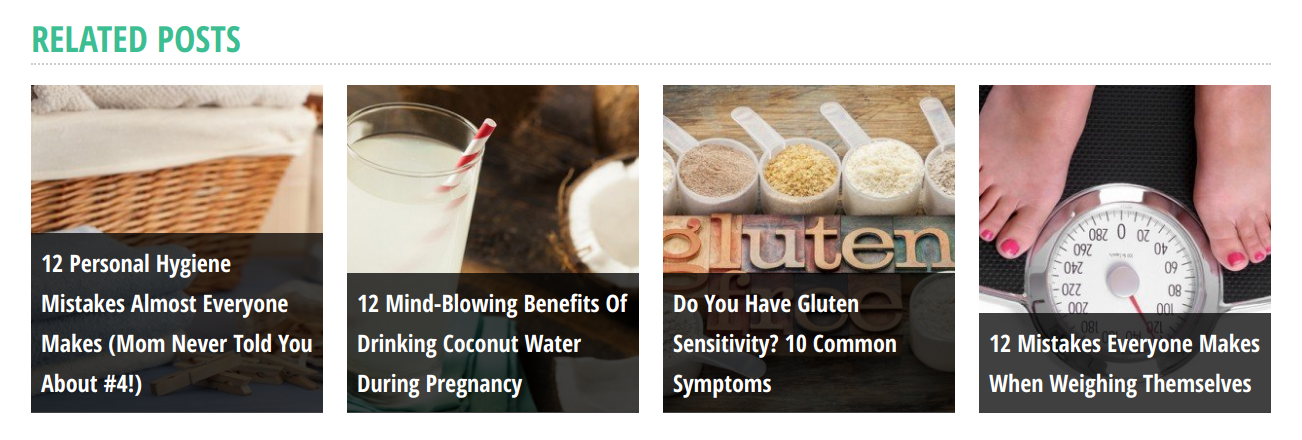
\includegraphics[width=\linewidth]{images/clickbait.png}
  \caption{Several clickbait articles in a 'chum box'}
  \label{fig:clickbait}
\end{figure}

\citeA{mahoney2015} terms a collection of clickbait stories as a 'chum boxes' - chum being dead fish used as bait for other fish. \citeauthor{mahoney2015} goes on to examine how clickbait uses psychological methods to manipulate, and how they can have an unconscious effect on an individual.

\paragraph{Fake News}
\citeA{allcott2017} defines fake news to be "news articles that are intentionally and verifiably false, and could mislead readers". For example, a fake news conspiracy theory claimed that a pizzeria, Comet Ping Pong, in Washington ran a child sex ring in its basement. Figure \ref{fig:fakenews} shows a news article from 2016 from Your News Wire\footnote{\url{https://archive.is/YTk3n}} (now News Punch).


\begin{figure}[ht!]
  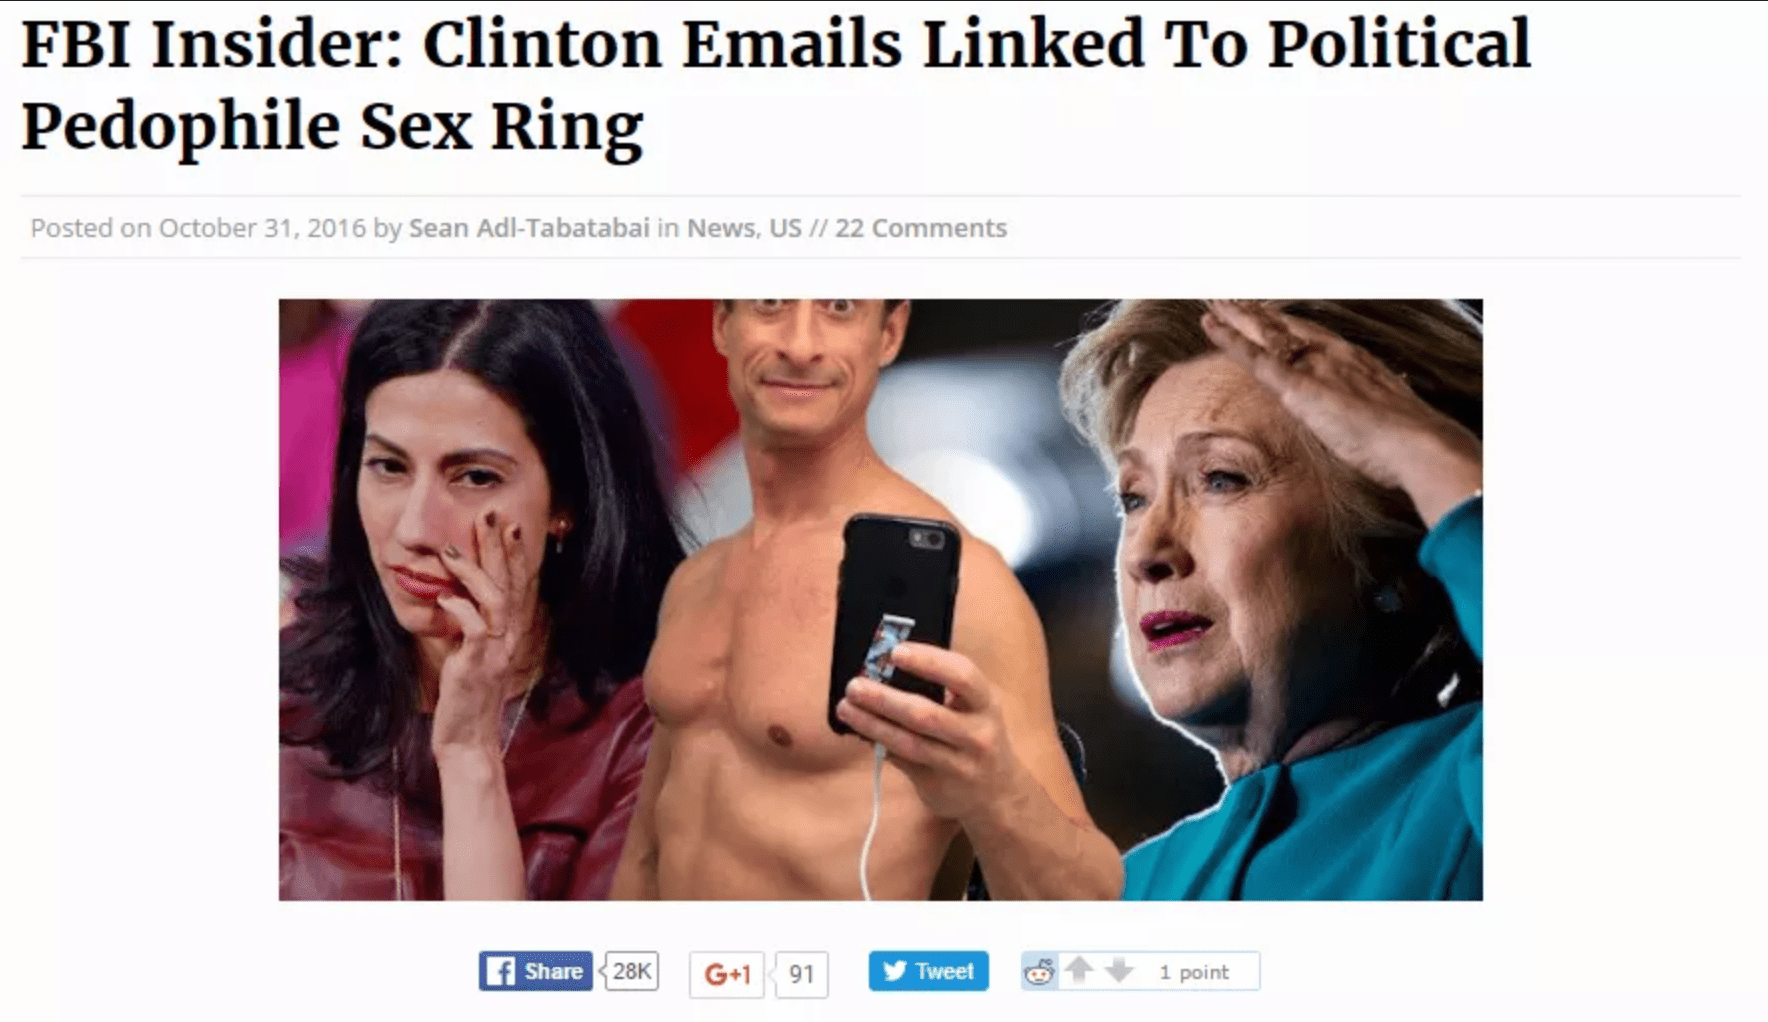
\includegraphics[width=\linewidth]{images/fakenews.png}
  \caption{A fake news story}
  \label{fig:fakenews}
\end{figure}


This lead to a man walking into Comet Ping Pong with an assault rifle and firing several shots. The restaurant's owner and staff also received several death threats \cite{lopez2016}. 

\citeauthor{allcott2017} go further in their definition, and give the following sub-categories for fake news: satire, parody, fabrication, manipulation, advertising and propaganda. While the intention of satire and parody is not to deceive but to criticise, the other classifications have more subversive aims, such as misinforming people or gaining as many clicks as possible.

\paragraph{Sensationalism}
\citeA{molek2013} defines sensationalism as "a specific discourse strategy  aimed  at  channeling  audience's  attention,  which  may  well  be  resorted  to  by  both  popular and quality outlet". They suggest that media fails to provide important and valuable news, in preference for that which is superficial and quick-paced.


Below are examples of sensationalised headlines, sourced from The Sun:

\begin{itemize}
	\item DOOMSDAY DISEASE FEARS Terrorists could turn ‘sniff and die’ virus that kills victims in 24 hours into a BIO-WEAPON
	\item SPICE UP YOUR LIFE Chilli and ginger ‘slash the risk of cancer – stopping tumours growing’
	\item JAB DEBATE As Melinda Messenger slams the HPV jab the parents of two teenagers blame their daughters’ ‘paralysis on vaccine’
	\item 'I KNOW WHO KILLED JONBENET' Juror from the JonBenet Ramsey case gives sensational interview revealing he ‘knows who killed six-year-old’
	
\end{itemize}

These headlines use dramatic language ('slams', 'sensational', 'slash') to evoke a sense of urgency and excitement in the reader, urging them to click through to the rest of the article. Unlike clickbait headlines, information is not withheld but rather dramatised - while the aim is still to get as many clicks as possible, this is achieved through different means.

This sensationalism is intended to provoke and entertain, at times at the expense of accuracy \cite{chesney2017}.

\subsubsection{Project scope}
This project will not consider fake news - by its nature, the entirety of a fake news article will be false, not just the headline. Therefore, to determine whether an article is fake, external sources would have to be consulted. Creating an algorithm for the truth, while an open problem in computer science\footnote{\url{https://www.youtube.com/watch?v=leX541Dr2rU}}, is considered out of the scope of this project.

Instead, this study will seek to evaluate to what extent a headline represents an article's body. This could identify sensationalism, over-exaggerated news stories and potentially some types of clickbait.

\subsection{Impact of Incongruence}
\citeA{karlsson2010} categorise online news both by its immediacy and interactivity, which has shortened the news cycle and increased the competitivity between publishers. Therefore, publishers have to make the news more appealing to potential consumers.

In the information-overload arena of online news reporting, the body of a news article is less read than the headline \cite{gabielkov2016}.  

For those that read beyond the headlines, incongruent articles can still be problematic; it's a well-established theory in psychology that first opinions matter \cite{digirolamo1997}. \citeA{ecker2014} ran a study that investigated how headlines affect the processing of the facts in news "Information that is initially accepted as valid but is later found to be incorrect can have a persistent influence on people’s memory and reasoning". Publishers can seek to sway individuals by using choice phrases to influence their mindset, which means that the same content could be interpreted in many ways depending on its headline \cite{reis2015}.

This means that if a headline is incongruent, even if the individual reads the whole article, there's a real possibility they will be left with a false impression of the facts. 


\subsection{Existing Approaches}

\citeA{manjesh2017} used a range of different techniques to identify clickbait and were able to achieve a 98\% accuracy with a deep learning approach. However, they only analysed the article's headline and disregarded the body text.  They found that clickbait headlines tend to have elaborate sentences with various linguistic nuances, such as "21 Pics Of Celebs Photoshopped In The Best Way Ever. These Are EPIC". There's also a statement at the end to further strengthen the main claim of the headline.

\citeA{park2020} used a deep learning approach to create a web interface for detecting incongruent articles. They managed to gain an accuracy of 86\%. However, for their dataset, they generated incongruent articles by swapping a completely different article's text in for the original. For example Headline A would have a section of Article B's body. They then considered congruent headlines to be those with the original body text in place. This could lead to false positives, and as the manufactured dataset does not reflect the incongruence in real-world articles their algorithm's output lacks validity.

The first Fake News Challenge (FNC1) was held by \citeA{pomerleaurao2017}. The challenge supplied a dataset of articles, and encouraged contestants to create a classifier capable of detecting fake news. While there has not been subsequent challenges, 50 teams competed and produced a wide range of different approaches. 

\subsection{Natural Language Processing}
Natural language processing (NLP) is a method of extracting information from a spoken or written language. 'Natural' here means the more free and less well defined human language, as opposed to strictly interpreted programming and mathematical notation. \cite{jackson2002}

 As natural language is filled with a range of nuances, assumptions and relies heavily on context, codifying it into a standardised, programmatic output poses a range of difficulties. For example, consider the following two sentences:

\begin{itemize}
	\item Apple's shares fell by 10\% in the last quarter
	\item An apple a day keeps the doctor away
\end{itemize}

The word 'apple' appear in both sentences, but in one it refers to a multinational company, and in the other a tasty fruit. It is only by using the context clues in the surrounding sentence that the meaning of the word can be deduced.

There are a range of different approaches that seek to tackle the problems inherent in determining the meaning and sentiment of natural language, each with their  characteristics, strengths and limitations. 

\subsubsection{Statistical NLP}
Statistical NLP creates metadata from a sentence and aims to extract meaning by using statistical inference \cite{manning1999}. Several techniques and models are used to create and interpret the metadata.

\paragraph{Tokens}
A token is typically an alphanumeric string or a punctuation mark. For instance, the sentence "Is this the way to Amarillo?" could be tokenised (represented as a list of tokens) like so: \texttt{"Is", "this", "the", "way", "to", "Amarillo", "?"}.\par
	
\paragraph{n-grams}
An n-gram is a subsection of a tokenised sentence, where \texttt{n} represents the number of tokens in a subsection. An n-gram of length 3 (also known as a tri-gram) of the above sentence could be \texttt{"way", "to", "Amarillo"}
	The location of these n-grams, their frequency and their composure all provide data points that can provide insights into the meaning of a body of text \cite{banerjee2003}.
	
\paragraph{Colocations}
\citeauthor{manning1999} describe a colocation as "an expression consisting of two or more words that correspond to some conventional way of saying things". For example, "around about", "stark naked" and "stiff upper lip" are all colocations. In a colocation, the subsequent parts make up a whole and lose some of their independent meaning - "fool hearted" makes sense to an English speaker's ear, but "idiot hearted" could sound offensive, or cause a misunderstanding.
	One way of identifying colocations is to count the frequency of bigrams in a body of text - a high number of two words occurring next to each other could indicate a colocation.

\paragraph{Hidden Markov Models} A Hidden Markov Model (HMM) is a system with hidden states. The system is comprised of a Markov chain, a model describing the probabilities an event occours. In NLP, HMMs can be used to identify how often a token or n-gram  


\subsubsection{Sentiment Analysis}
Sentiment analysis is a branch of NLP that could potentially aid the detection of an incongrous article. It's a relatively new development (no substantial research had been conducted before 2000) that aims to extract opinions from text and speech \cite{liu2012}.

\citeA{liu2012} identifies a key problem with sentiment analysis: sentiment is a very subjective concept, and calculating an absolute sentiment score for a sentence is fraught with potential difficulties. For instance, the phrase "I really enjoy writing in an academic style" could be interpreted as a very positive remark, or perceived with sarcastic overtones and classified as a negative sentiment.

Sentiment analysis could be used to approach this project - both the headline and the body could be analyised, and the results compared. The difference in sentiment could then be used as an incongruence score.

\subsubsection{Stance Detection}


